\documentclass[a4paper,14pt]{extarticle}
% ================== ОФОРМЛЕНИЕ ==================
\usepackage[T2A]{fontenc}
\usepackage[utf8]{inputenc}
\usepackage[russian]{babel}
\usepackage[left=30mm,right=15mm,top=20mm,bottom=20mm]{geometry}
\usepackage{amsmath,amssymb}
\usepackage{graphicx}
\usepackage{float}
\usepackage{booktabs}
\usepackage{array}
\usepackage{caption}
\usepackage{indentfirst}
\usepackage{hyperref}
\hypersetup{hidelinks}
% microtype намеренно не используется: это предотвращает
% ошибку font expansion на некоторых установках TeX Live.
\setlength{\parindent}{1.25cm}
\setlength{\parskip}{0pt}
\linespread{1.08}
\renewcommand{\arraystretch}{1.15}
\setlength{\emergencystretch}{2em}
\addto\captionsrussian{\renewcommand{\figurename}{Рис.}}
\captionsetup{font=small,labelfont=normalfont,labelsep=colon}
\begin{document}
% ================== ТИТУЛЬНЫЙ ЛИСТ ==================
\hypersetup{pageanchor=false}
\begin{titlepage}
\thispagestyle{empty}
\begin{center}
  \vspace*{0cm}
  {\normalsize Московский Физико-Технический Институт\par}
  \vspace{3cm}
  {\normalsize Лабораторная работа №3.2.4, №3.2.5\par}
  \vspace{0.65cm}
  \rule{\textwidth}{0.4pt}
  \vspace{0.30cm}
  {\bfseries\LARGE
    Свободные и вынужденные колебания\\
    в электрическом контуре\par}
  \vspace{0.34cm}
  \rule{\textwidth}{0.4pt}
\end{center}

\vspace{6.1cm}
\hfill
\begin{minipage}{0.42\textwidth}
  \raggedright
  Выполнил:\\
  Студент 2 курса ФАКТ\\
  Группа Б03-502\\
  Подмосковнов Лев
\end{minipage}

\vfill
\begin{center}
  Долгопрудный\\
  2026
\end{center}

\end{titlepage}

\hypersetup{pageanchor=true}
\setcounter{page}{1}
% ================== ЦЕЛЬ И ПРИБОРЫ ==================

\section*{Цель работы}
Исследование свободных и вынужденных колебаний в колебательном контуре.

\section*{Используемые приборы и материалы}
\begin{itemize}
  \item осциллограф АКТАКОМ ADS-6142H;
  \item генератор сигналов специальной формы АКИП-3409/4;
  \item магазин сопротивлений МСР-60;
  \item магазин ёмкостей Р5025;
  \item магазин индуктивностей Р567 (МИСП);
  \item соединительная коробка с шунтирующей ёмкостью;
  \item соединительные одножильные и коаксиальные провода.
\end{itemize}

% ================== ТЕОРИЯ ==================

\section{Теоретическое введение}

\subsection{Свободные затухающие колебания}
Колебательный контур содержит индуктивность $L$, ёмкость $C$ и
активное сопротивление $R$. Дополнительно учитываются активное
сопротивление катушки $R_L$ и собственная ёмкость установки $C_0$.
Для расчётов используются полные значения
\begin{equation}
  C_\Sigma=C+C_0, \qquad R_\Sigma=R+R_L.
\end{equation}

Короткий импульс генератора заряжает конденсатор. Затем между
импульсами в контуре наблюдаются свободные затухающие колебания.
В приближении слабого затухания собственная частота и период равны
\begin{equation}
  \nu_0=\frac{1}{2\pi\sqrt{LC_\Sigma}},\qquad
  T_\text{теор}=2\pi\sqrt{LC_\Sigma}.
\end{equation}

Логарифмический декремент затухания определяется по амплитудам,
разделённым целым числом периодов $n$:
\begin{equation}
  \Theta=\frac{1}{n}\ln\frac{U_m}{U_{m+n}}.
\end{equation}

Критическое сопротивление, при котором колебательный режим
переходит в апериодический, составляет
\begin{equation}
  R_\text{кр}=2\sqrt{\frac{L}{C_\Sigma}}.
\end{equation}

Добротность контура в приближении слабого затухания:
\begin{equation}
  Q\simeq\frac{\pi}{\Theta}.
\end{equation}


\subsection{Вынужденные колебания и резонанс}
При подаче синусоидального сигнала возбуждаются вынужденные
колебания. Зависимость их амплитуды от частоты генератора
называется амплитудно-частотной характеристикой (АЧХ),
а зависимость разности фаз --- фазочастотной характеристикой (ФЧХ).
При выбранном знаке $\Delta t>0$ для запаздывающего напряжения
разность фаз определяется по временному сдвигу сигналов:
\begin{equation}
  \Delta\varphi=-2\pi\nu\Delta t.
\end{equation}

Добротность можно определить по полной ширине резонансной
кривой $2\Delta\Omega$ на уровне $U_0/\sqrt{2}$:
\begin{equation}
  Q_\text{АЧХ}=\frac{\omega_0}{2\Delta\Omega}.
\end{equation}

По ФЧХ добротность определяется методом, описанным в методичке,
с использованием частотного интервала $\Delta\omega$:
\begin{equation}
  Q_\text{ФЧХ}=\frac{\omega_0}{\Delta\omega}.
\end{equation}


\subsection{Установление и затухание вынужденных колебаний}
При подаче цугов синусоидальных колебаний можно отдельно наблюдать
рост амплитуды и её последующее затухание. Для нарастающего участка
логарифмический декремент определяется выражением
\begin{equation}
  \Theta_\text{нар}=\frac{1}{n}
  \ln\frac{U_0-U_k}{U_0-U_{k+n}},
\end{equation}

где $U_0$ --- установившаяся амплитуда.
Для участка затухания применяется формула
\begin{equation}
  \Theta_\text{зат}=\frac{1}{n}\ln\frac{U_m}{U_{m+n}}.
\end{equation}

% ================== СВОБОДНЫЕ КОЛЕБАНИЯ ==================

\section{Исследование свободных колебаний}

\subsection{Измерение периода при изменении ёмкости}
При фиксированной индуктивности $L=100$~мГн и $R=0$~Ом
измерялся период затухающих колебаний при изменении показания
магазина ёмкостей от $0$ до $0{,}009$~мкФ.
Период при $C=0$ использовался для определения
собственной ёмкости контура:
\begin{equation}
    C_0 = \frac{T_0^2}{4\pi^2 L}.
\end{equation}

Измеренный период составляет $T_0 = 65$ мкс.
При $L = 100$ мГн получаем:
\begin{equation}
    C_0 = \frac{(65\cdot10^{-6})^2}
    {4\pi^2\cdot0{,}1}
    \approx 0{,}00107\text{ мкФ}.
\end{equation}

\begin{table}[H]
\centering
\small
\caption{Период свободных колебаний при различных ёмкостях}
\begin{tabular}{cccc}
\toprule
$C$, мкФ &
$C_\Sigma$, мкФ &
$T_{\text{эксп}}$, мкс &
$T_{\text{теор}}$, мкс \\
\midrule
0,001 & 0,00207 & 90  & 90,40  \\
0,002 & 0,00307 & 110 & 110,09 \\
0,003 & 0,00407 & 128 & 126,76 \\
0,004 & 0,00507 & 146 & 141,48 \\
0,005 & 0,00607 & 156 & 154,80 \\
0,006 & 0,00707 & 166 & 167,07 \\
0,007 & 0,00807 & 180 & 178,49 \\
0,008 & 0,00907 & 190 & 189,23 \\
0,009 & 0,01007 & 200 & 199,39 \\
\bottomrule
\end{tabular}
\end{table}

\begin{figure}[H]
    \centering
    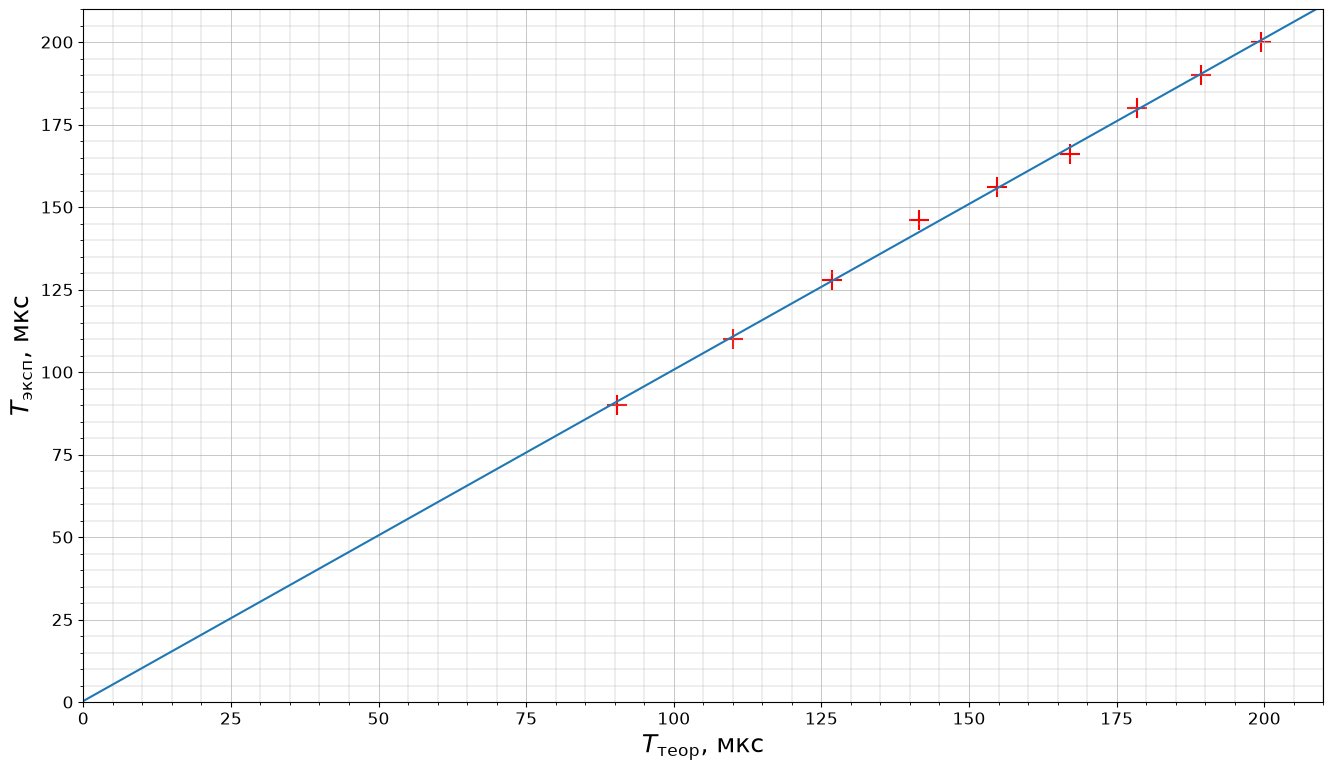
\includegraphics[width=0.85\textwidth]{figures/period.png}
    \caption{Зависимость экспериментального периода
    свободных колебаний ($T_{\text{эксп}}$) от теоретического ($T_{\text{теор}}$)}
    \label{fig:period}
\end{figure}

Из графика получена линейная зависимость
\[
    T_{\text{эксп}} =
    (1{,}004 \pm 0{,}016)T_{\text{теор}}
    + (0{,}31 \pm 2{,}52)\text{ мкс}.
\]

Полученные коэффициенты согласуются с теоретическими
значениями $a=1$ и $b=0$ в пределах погрешности.
Таким образом, эксперимент подтверждает формулу Томсона:
\begin{equation}
    T = 2\pi\sqrt{LC_\Sigma}.
\end{equation}


\subsection{Критическое сопротивление контура}
При $L=100$ мГн и заданной собственной частоте
$\nu_0=6{,}5$ кГц требуемая полная ёмкость составляет
\[
    C^*=\frac{1}{(2\pi\nu_0)^2 L}\approx6{,}00\text{ нФ}.
\]

При установленной на магазине ёмкости $C=6{,}00$ нФ
следует учитывать собственную ёмкость установки $C_0=1{,}07$ нФ:
\[
    C_\Sigma=C+C_0=7{,}07\text{ нФ}.
\]

Для фактически установленной полной ёмкости теоретическое
критическое сопротивление составляет
\[
    R_{\text{кр,теор}}=2\sqrt{\frac{L}{C_\Sigma}}
    \approx7522\text{ Ом}.
\]

Переход к апериодическому режиму наблюдался при показании
магазина сопротивлений $R=6000$ Ом. С учётом активного
сопротивления катушки $R_L=200{,}26$ Ом получаем
\[
    R_{\text{кр,эксп}}=R+R_L=6200{,}26\text{ Ом}.
\]

Относительное отличие от расчётного значения составляет
\[
    \varepsilon_{\text{кр}}=
    \frac{|6200{,}26-7522|}{7522}\cdot100\%\approx17{,}6\%.
\]


\subsection{Логарифмический декремент затухания}
Активное сопротивление катушки $R_L=200{,}26$ Ом, поэтому
$R_\Sigma=R+R_L$.
Для различных значений сопротивления измерялись
амплитуды двух соседних максимумов затухающих
колебаний $U_1$ и $U_2$.
Поскольку $n=1$, логарифмический декремент
затухания определялся по формуле
\begin{equation}
    \Theta = \ln\frac{U_1}{U_2}.
\end{equation}

\begin{table}[H]
\centering
\small
\caption{Измерение логарифмического декремента затухания}
\begin{tabular}{ccccc}
\toprule
$R$, Ом &
$R_\Sigma$, Ом &
$U_1$, мВ &
$U_2$, мВ &
$\Theta$ \\
\midrule
400  & 600,26 & 580 & 392 & 0,3918 \\
640  & 840,26 & 500 & 280 & 0,5798 \\
800  & 1000,26 & 444 & 220 & 0,7022 \\
960  & 1160,26 & 408 & 176 & 0,8408 \\
1200 & 1400,26 & 356 & 128 & 1,0229 \\
1440 & 1640,26 & 308 & 92  & 1,2083 \\
1600 & 1800,26 & 284 & 76  & 1,3182 \\
1760 & 1960,26 & 256 & 60  & 1,4508 \\
2000 & 2200,26 & 216 & 44 & 1,5911 \\
\bottomrule
\end{tabular}
\end{table}

Для дальнейшего исследования выбраны
$R_1=400$~Ом и $R_2=2000$~Ом.
\begin{figure}[H]
    \centering
    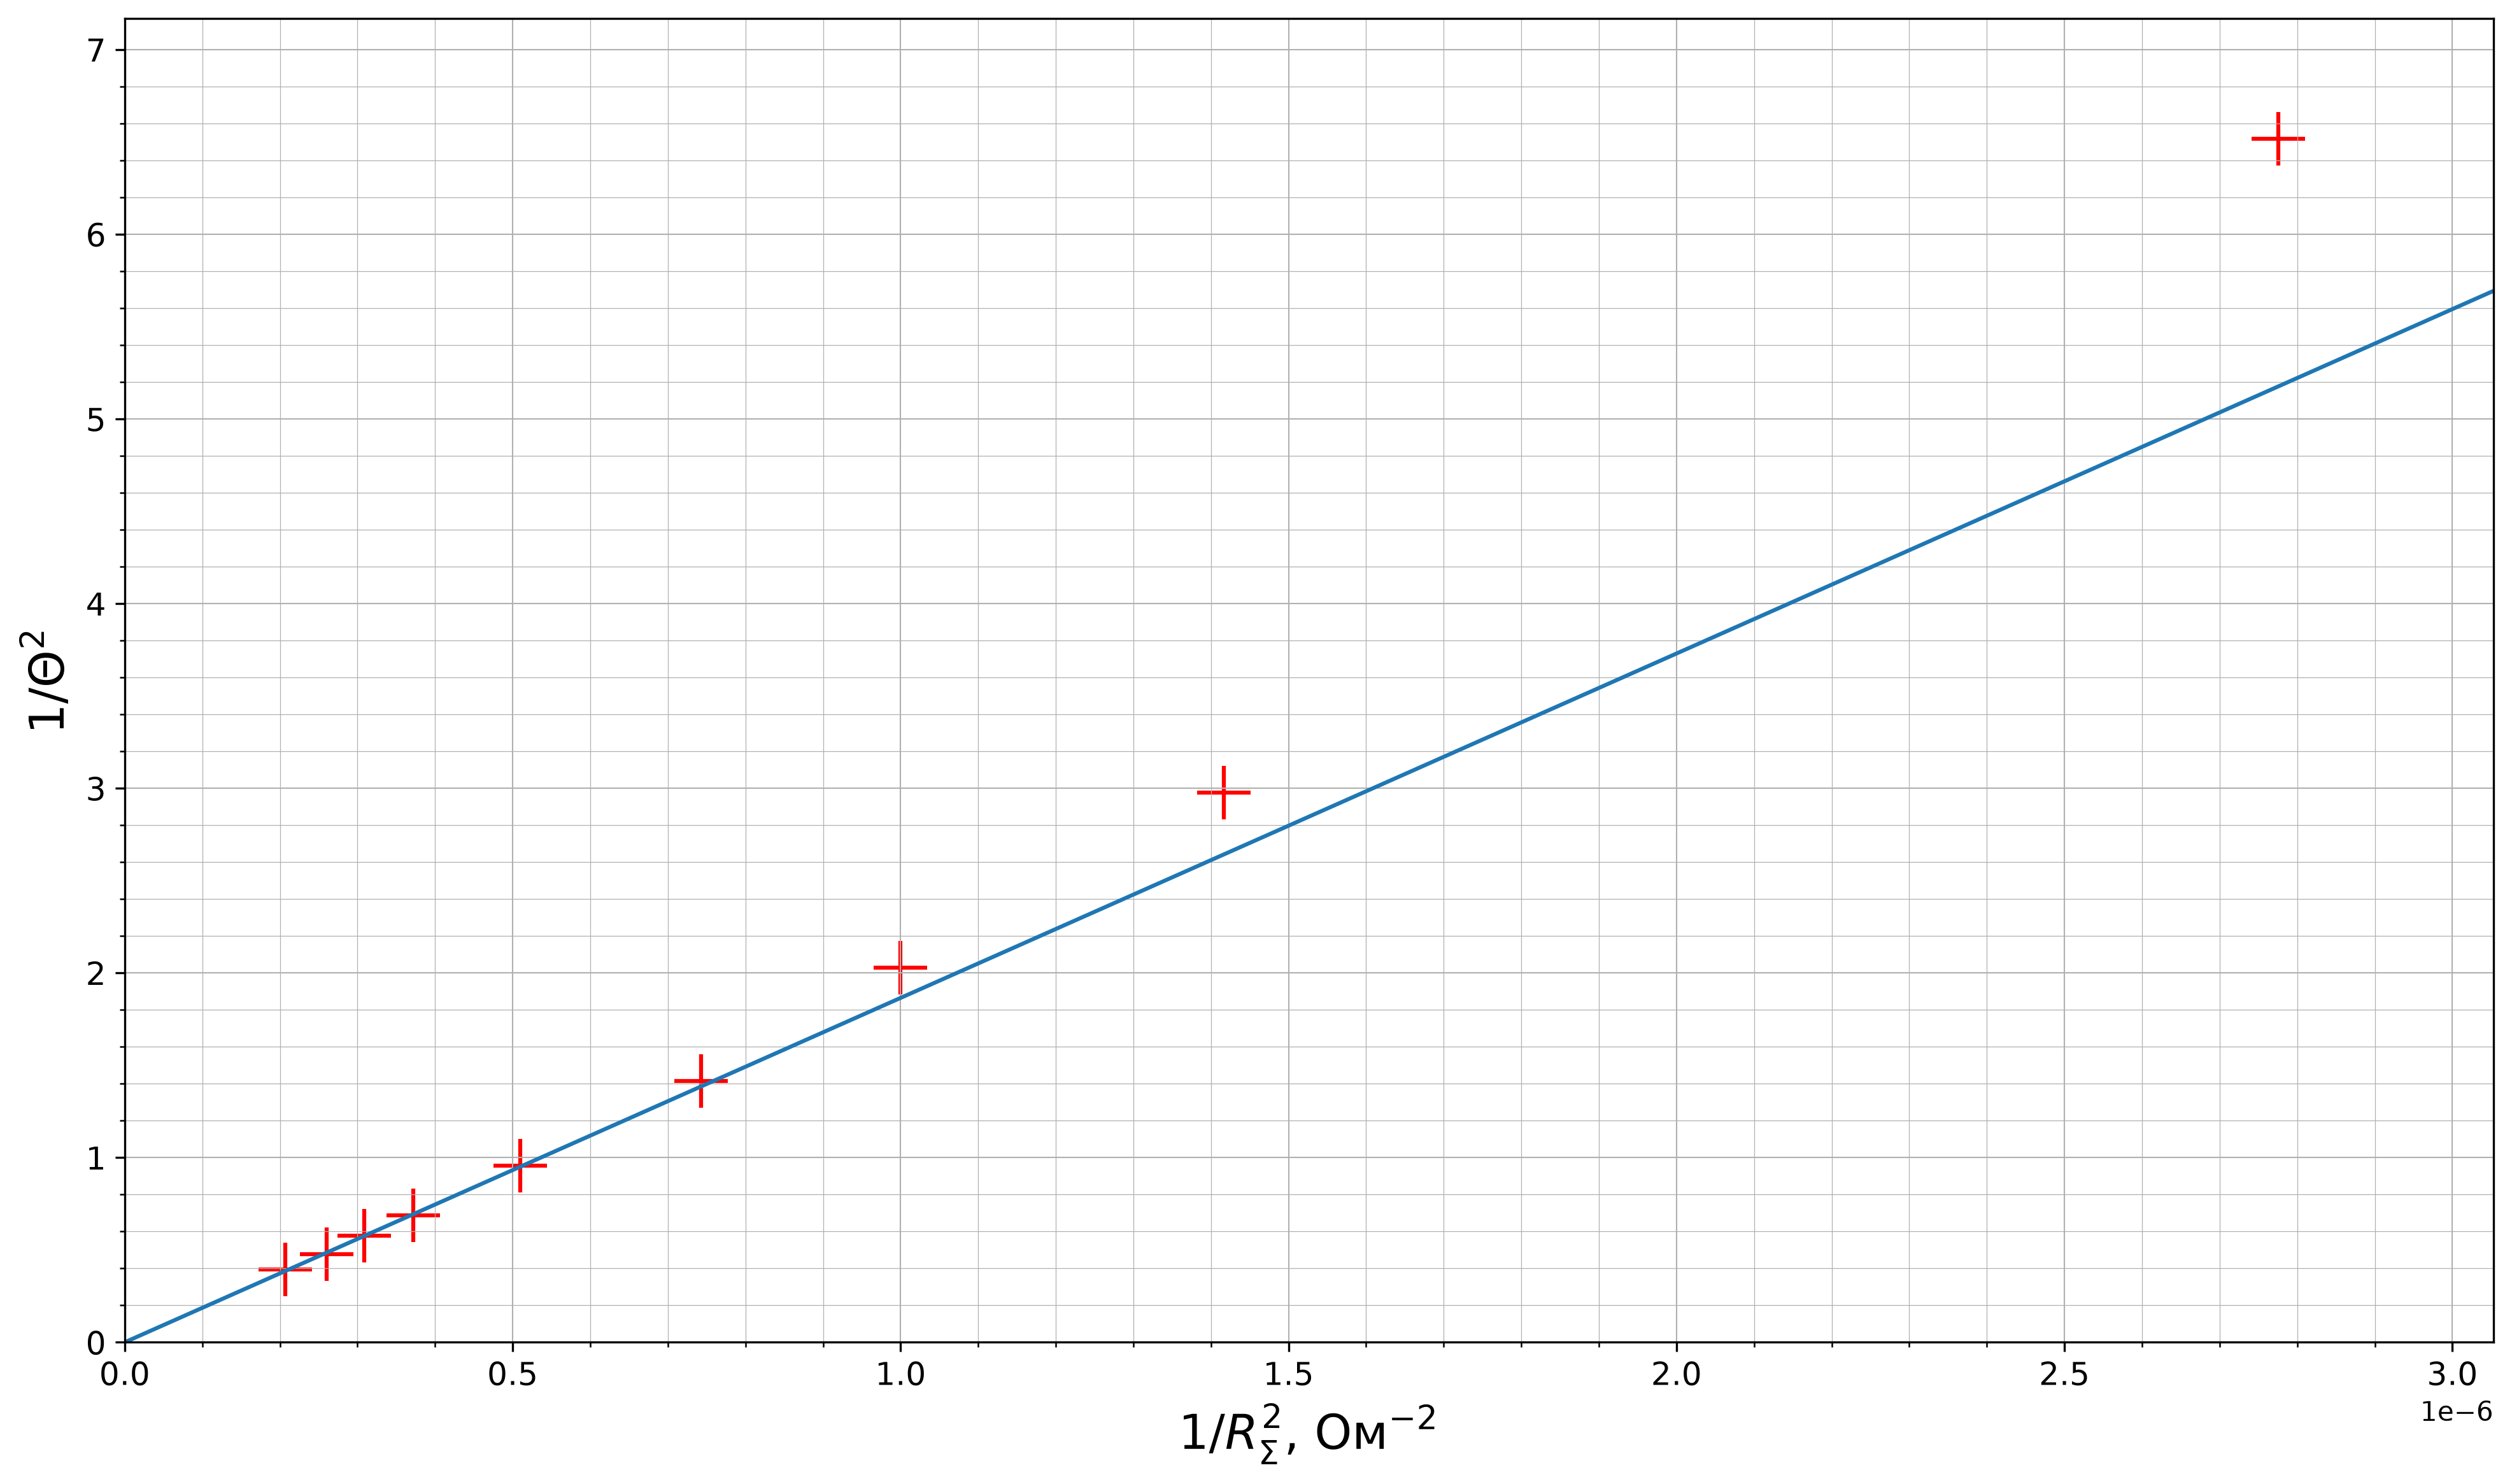
\includegraphics[width=0.85\textwidth]{figures/inv_theta_inv_r2.png}
    \caption{Зависимость обратного квадрата логарифмического
    декремента затухания ($1/\Theta^2$) от обратного квадрата
    полного сопротивления контура ($1/R_\Sigma^2$)}
    \label{fig:inv_theta_inv_r2}
\end{figure}

По пяти точкам, ближайшим к началу координат, линейная
аппроксимация дала коэффициент наклона
\[
    a=(1{,}865\pm0{,}042)\cdot10^6\text{ Ом}^2.
\]

Критическое сопротивление, рассчитанное по наклону графика,
равно
\[
    R_{\text{кр,гр}}=2\pi\sqrt{a}
    =(8580\pm96)\text{ Ом}.
\]

Графическое значение отличается от расчётного
$R_{\text{кр,теор}}=7522$ Ом на $14{,}1\%$,
что превышает статистическую погрешность аппроксимации.

\subsection{Добротность по свободным колебаниям}
Добротность контура определяется по формуле
\[
    Q = \frac{\pi}{\Theta}.
\]

Для минимального и максимального значений
логарифмического декремента получаем:
\[
    Q_{\max} = \frac{\pi}{0{,}3918} \approx 8{,}02,
\]

\[
    Q_{\min} = \frac{\pi}{1{,}5911} \approx 1{,}97.
\]

Таким образом, при увеличении сопротивления
контура добротность уменьшается, что соответствует
более быстрому затуханию свободных колебаний.
\newpage

\subsection{Свободные колебания на фазовой плоскости}
При наблюдении свободных затухающих колебаний
в режиме XY осциллографа была получена фазовая
траектория в виде спирали.
\begin{figure}[H]
    \centering
    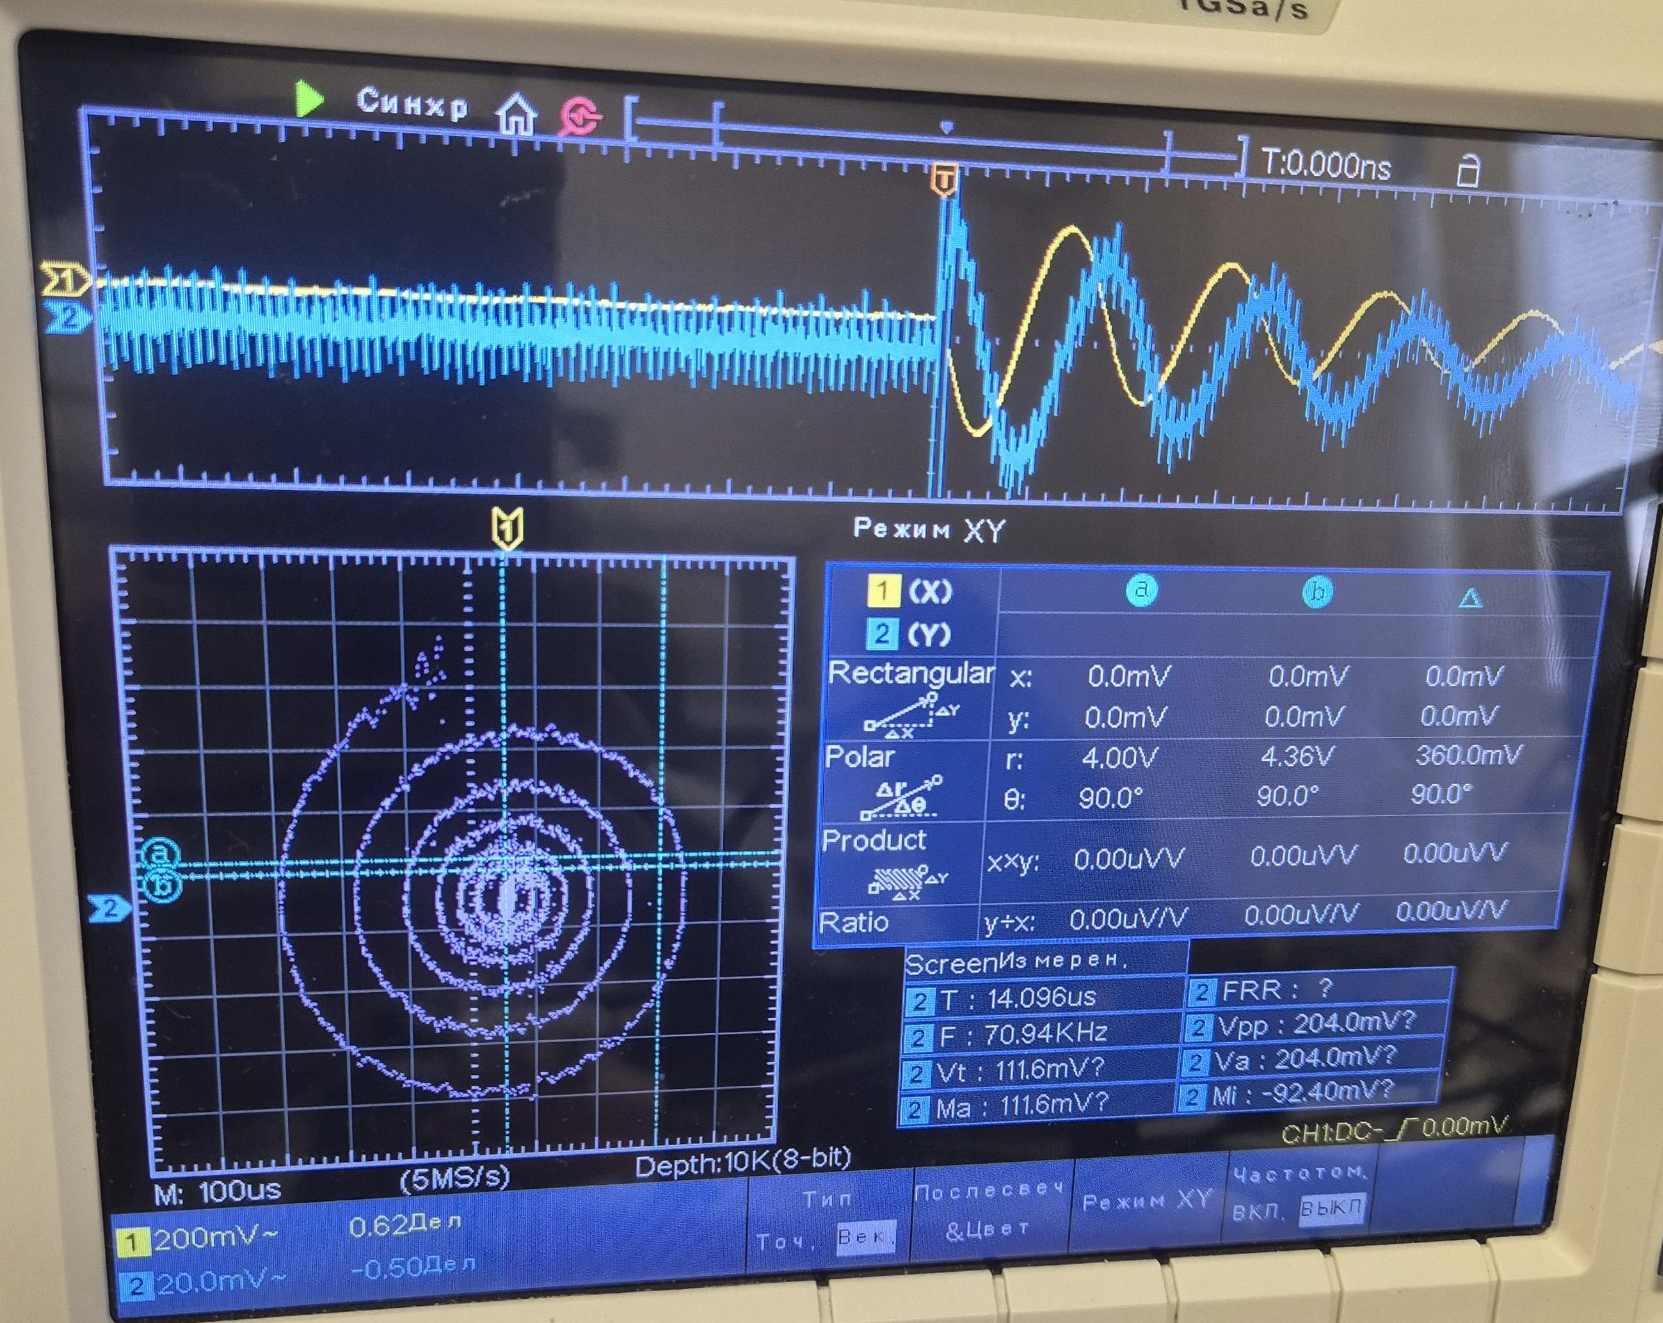
\includegraphics[width=0.85\textwidth]{figures/spiral.png}
    \caption{Фазовая спираль свободных затухающих колебаний}
    \label{fig:spiral}
\end{figure}

По мере затухания колебаний радиус фазовой
спирали уменьшается, что соответствует
уменьшению амплитуд напряжения и тока.
\begin{table}[H]
\centering
\small
\caption{Расчёт добротности по фазовым траекториям}
\begin{tabular}{ccccc}
\toprule
$R$, Ом &
$U_1$, мВ &
$U_2$, мВ &
$\Theta$ &
$Q$ \\
\midrule
400 & 24,8 & 16,8 & 0,3895 & 8,07\\
640 & 22,8 & 12,8 & 0,5773 & 5,44\\
800 & 18,4 & 9,1 & 0,7041 & 4,46\\
960 & 15,2 & 6,6 & 0,8342 & 3,77\\
1200 & 10,8 & 3,9 & 1,0186 & 3,08\\
1440 & 8,4 & 2,5 & 1,2119 & 2,59\\
\bottomrule
\end{tabular}
\end{table}

Для $R_1=400$ Ом получаем
$Q_{\text{сп},1}\approx8{,}07$.
При $R_2=2000$ Ом отдельных амплитуд с фазовой спирали
не представлено, поэтому значение этим способом не определено.
% ================== ВЫНУЖДЕННЫЕ КОЛЕБАНИЯ ==================

\section{Исследование вынужденных колебаний}

\subsection{Амплитудно-частотная и фазочастотная характеристики}
Измерялись амплитуда напряжения на конденсаторе $U_C$
и сдвиг сигналов $\Delta t$ в зависимости от частоты генератора.
В окрестности резонанса для каждого сопротивления необходимо
снять не менее десяти точек по обе стороны от максимума.

\subsection{Теоретическая добротность контура}
Теоретическая добротность контура определяется
по формуле
\[
    Q_{\text{теор}} =
    \frac{1}{R_\Sigma}\sqrt{\frac{L}{C_\Sigma}},
\]

где $R_\Sigma = R + R_L$ и $C_\Sigma = C + C_0$.
При $L = 0{,}1$ Гн, $C_\Sigma = 7{,}07$ нФ
и $R_L = 200{,}26$ Ом получаем:
\[
    Q_{\text{теор},1} =
    \frac{1}{600{,}26}
    \sqrt{\frac{0{,}1}{7{,}07\cdot10^{-9}}}
    \approx 6{,}27,
\]

\[
    Q_{\text{теор},2} =
    \frac{1}{2200{,}26}
    \sqrt{\frac{0{,}1}{7{,}07\cdot10^{-9}}}
    \approx 1{,}71.
\]

\newpage

\subsubsection*{Измерения при $R_1=400$~Ом}
\noindent $\nu_{0,1}=6{,}012$~кГц; $U_{0,1}=8{,}35$~В.
\begin{table}[H]
\centering
\small
\caption{Амплитуда и временной сдвиг
при $R=400$ Ом}
\begin{tabular}{ccc}
\toprule
$\nu$, кГц & $U_C$, В & $\Delta t$, мкс \\
\midrule
5,30 & 3,35 & 75,6 \\
5,37 & 3,75 & 75,6 \\
5,44 & 4,10 & 73,2 \\
5,51 & 4,45 & 69,2 \\
5,58 & 5,15 & 66,8 \\
5,65 & 5,70 & 62,8 \\
5,72 & 6,45 & 58,8 \\
5,79 & 7,15 & 54,8 \\
5,86 & 7,75 & 49,2 \\
5,93 & 8,25 & 43,2 \\
6,00 & 8,30 & 38,4 \\
6,07 & 8,25 & 33,4 \\
6,14 & 8,00 & 28,4 \\
6,21 & 7,55 & 24,5 \\
6,28 & 7,00 & 21,2 \\
6,35 & 6,45 & 18,6 \\
6,42 & 5,90 & 16,0 \\
6,49 & 5,40 & 14,1 \\
6,56 & 5,10 & 12,4 \\
6,63 & 4,80 & 10,1 \\
6,70 & 4,55 & 8,8  \\
\bottomrule
\end{tabular}
\end{table}

\newpage

\subsubsection*{Измерения при $R_2=2000$~Ом}
\noindent $\nu_{0,2}=6{,}00$~кГц; $U_{0,2}=2{,}20$~В.
\begin{table}[H]
\centering
\small
\caption{Амплитуда и временной
сдвиг при $R=2000$ Ом}
\begin{tabular}{ccc}
\toprule
$\nu$, кГц & $U_C$, В & $\Delta t$, мкс \\
\midrule
5,30 & 1,91 & 48,8 \\
5,37 & 1,95 & 47,3 \\
5,44 & 1,98 & 45,5 \\
5,51 & 2,02 & 43,5 \\
5,58 & 2,05 & 41,5 \\
5,65 & 2,08 & 39,7 \\
5,72 & 2,11 & 37,7 \\
5,79 & 2,14 & 35,7 \\
5,86 & 2,16 & 33,9 \\
5,93 & 2,18 & 32,2 \\
6,00 & 2,20 & 30,5 \\
6,07 & 2,19 & 28,9 \\
6,14 & 2,18 & 27,4 \\
6,21 & 2,16 & 25,9 \\
6,28 & 2,14 & 24,6 \\
6,35 & 2,12 & 23,3 \\
6,42 & 2,09 & 22,1 \\
6,49 & 2,06 & 20,9 \\
6,56 & 2,03 & 19,8 \\
6,63 & 2,00 & 18,7 \\
6,70 & 1,97 & 17,7 \\
\bottomrule
\end{tabular}
\end{table}

\newpage

\subsection{Исследование резонансных кривых}
Построены нормированные амплитудно-частотные
характеристики контура при различных сопротивлениях.
\begin{figure}[H]
    \centering
    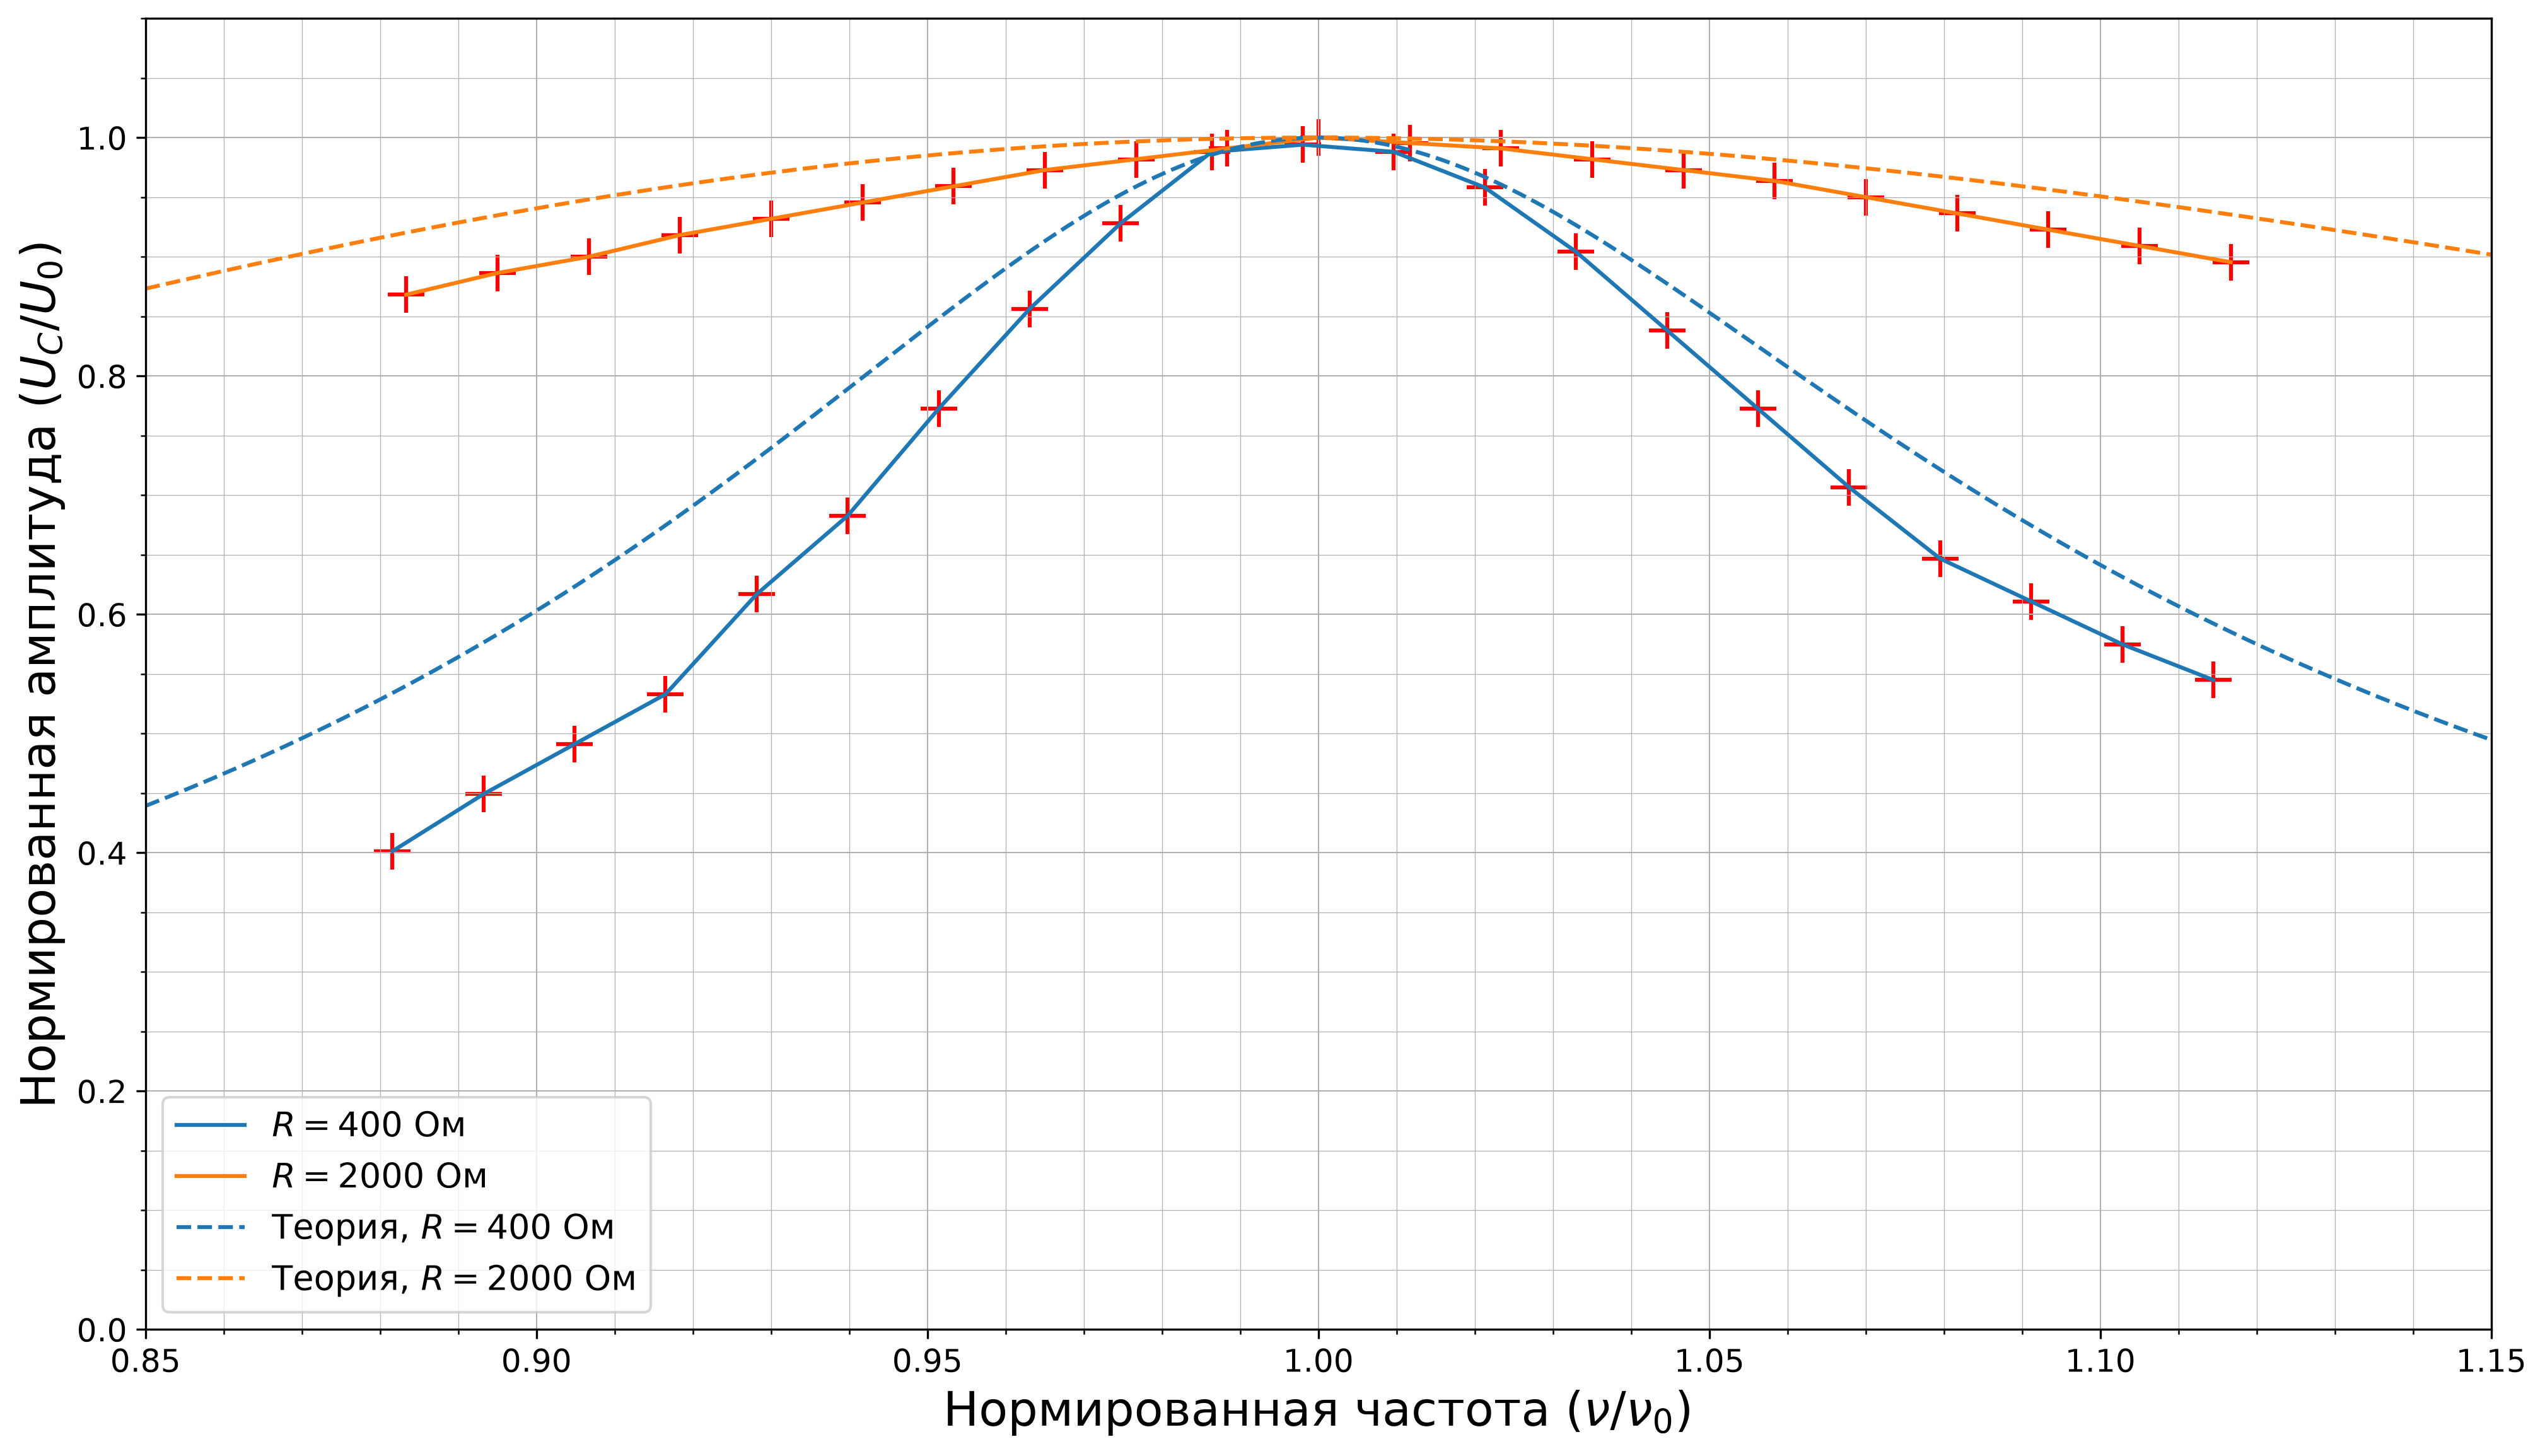
\includegraphics[width=0.85\textwidth]{figures/achx.png}
    \caption{Зависимость нормированной амплитуды
    напряжения ($U_C/U_0$) от нормированной
    частоты ($\nu/\nu_0$) при различных сопротивлениях}
    \label{fig:achx}
\end{figure}

Из графика видно, что при увеличении сопротивления
резонансная кривая становится более пологой.
Это соответствует уменьшению добротности
колебательного контура.

\subsection{Определение добротности по АЧХ}
Добротность определяется по ширине резонансной
кривой на уровне $U_0/\sqrt{2}$:
\[
    Q_{\text{АЧХ}} =
    \frac{\omega_0}{2\Delta\Omega}.
\]

Для $R=400$ Ом получено:
\[
    \nu_- = 5{,}669\text{ кГц},
    \qquad
    \nu_+ = 6{,}419\text{ кГц}.
\]

Следовательно, полная ширина резонансной
кривой составляет
\[
    2\Delta\Omega =
    2\pi(\nu_+-\nu_-)
    \approx 4715\text{ рад/с},
\]

где частоты в расчёте переведены в герцы.
Таким образом,
\[
    Q_{\text{АЧХ},1} \approx 8{,}01.
\]

Для $R=2000$ Ом уровень $U_0/\sqrt2=1{,}56$ В
не пересекается с обеими ветвями АЧХ в исследованном диапазоне.
Для получения численной оценки проведена аппроксимация
нормированной характеристики выражением
\[
    \frac{U_C}{U_0}=\frac{1}{\sqrt{1+Q^2(x-x^{-1})^2}},
    \qquad x=\frac{\nu}{\nu_0}.
\]
По наименьшим квадратам получено
\[
    Q_{\text{АЧХ},2}\approx2{,}39.
\]
Для этого сопротивления численное значение получено
по аппроксимации кривой, а не по непосредственно измеренной ширине.

\subsection{Определение добротности по ФЧХ}
Для определения добротности нижняя часть
фазочастотной характеристики была отражена
относительно уровня $-\pi/2$.
\begin{figure}[H]
    \centering
    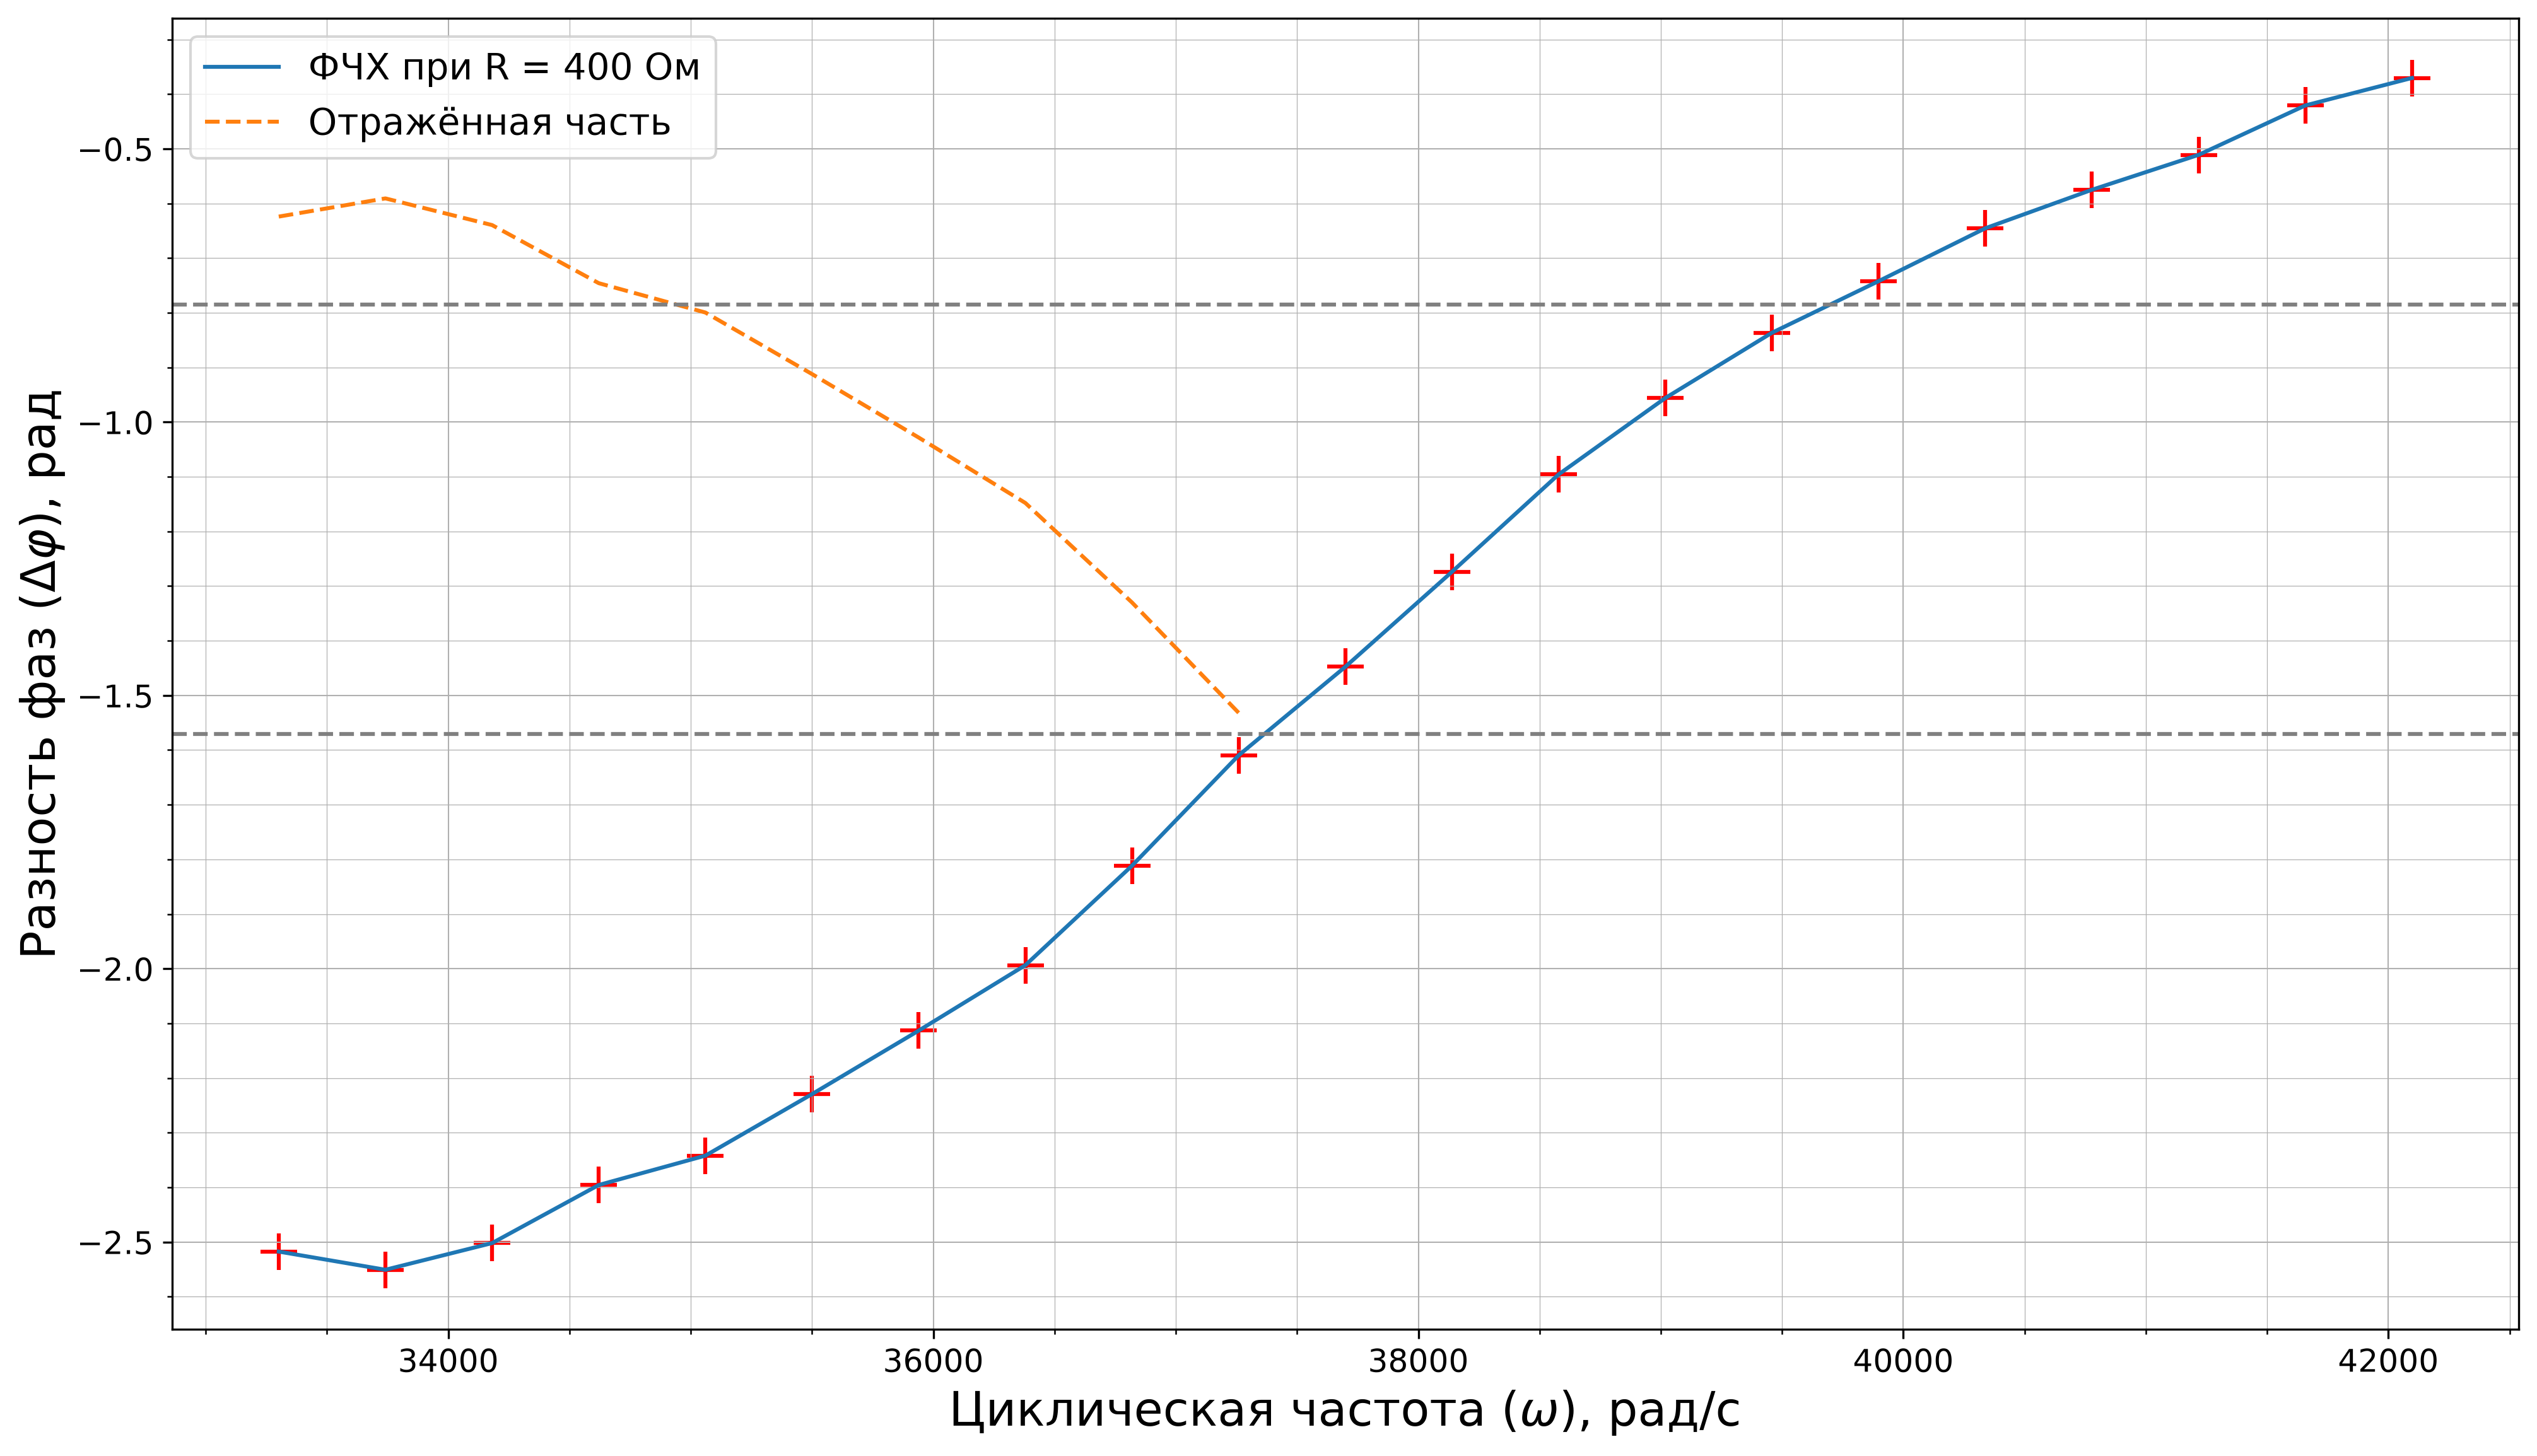
\includegraphics[width=0.85\textwidth]{figures/fchx_Q.png}
    \caption{Определение добротности по зависимости
    разности фаз ($\Delta\varphi$) от циклической
    частоты ($\omega$)}
    \label{fig:fchx_Q}
\end{figure}

Из графика определена ширина
фазочастотной характеристики на уровне $-\pi/4$:
\[
    \Delta\omega \approx 4752\text{ рад/с}.
\]

Добротность контура составляет
\[
    Q_{\text{ФЧХ},1} =
    \frac{\omega_0}{\Delta\omega}
    \approx 7{,}95.
\]

Полученное значение близко к добротности, определённой по амплитудно-частотной характеристике: $Q_{\text{АЧХ},1}=8{,}01$.

\subsection{Сравнение фазочастотных характеристик}
\begin{figure}[H]
    \centering
    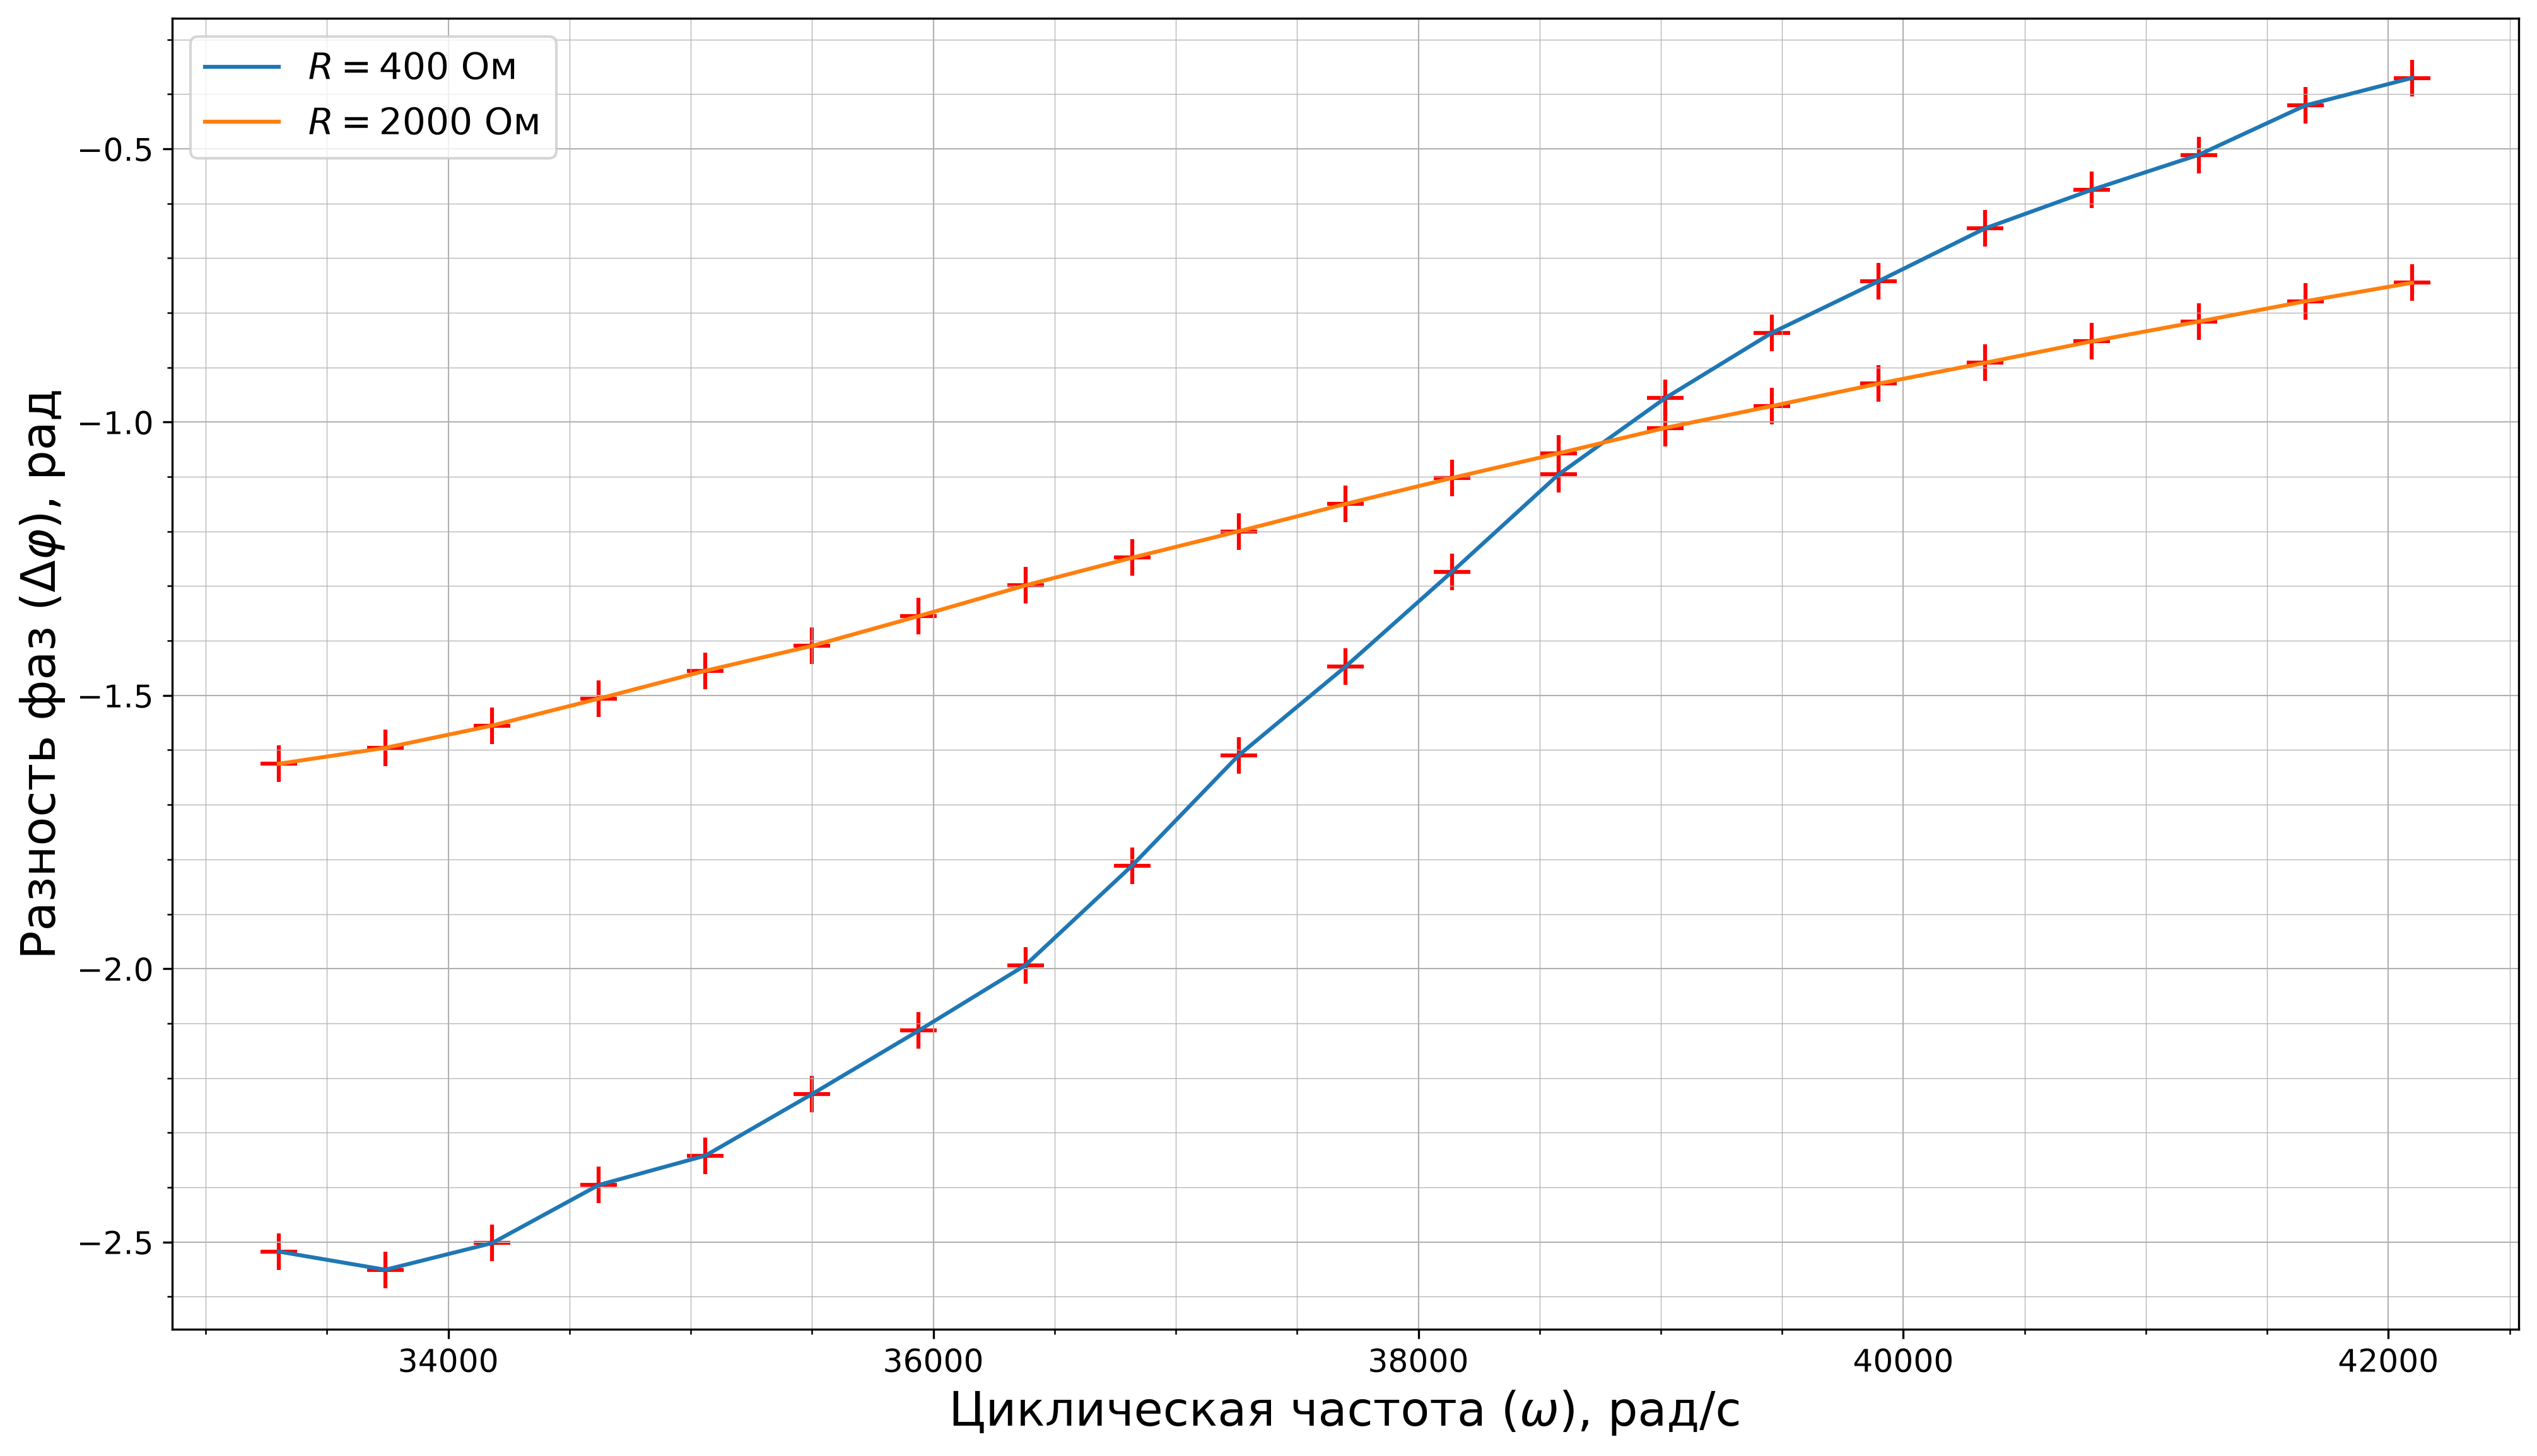
\includegraphics[width=0.85\textwidth]{figures/fchx.png}
    \caption{Зависимость разности фаз
    ($\Delta\varphi$) от циклической частоты
    ($\omega$) при различных сопротивлениях}
    \label{fig:fchx}
\end{figure}

Из графика видно, что при увеличении
сопротивления фазочастотная характеристика
становится более пологой, что соответствует
уменьшению добротности контура.
Для $R=2000$ Ом в снятом диапазоне нет пересечения с
уровнем $-3\pi/4$, необходимого для прямого применения
метода отражения. Для оценки добротности использована
аппроксимация фазовой зависимости выражением
\[
  \Delta\varphi(x)=\varphi_c+
    \arctan\!\left[Q(x-x^{-1})\right],
  \qquad x=\frac{\nu}{\nu_0},
\]
где $\varphi_c$ допускает постоянное смещение нуля фазы.
По табличным точкам получено
\[
   Q_{\text{ФЧХ},2}\approx2{,}05, \qquad
   \varphi_c\approx-1{,}16\text{ рад}.
\]
Это оценка по аппроксимации всей зависимости; значение
фазового смещения отличается от $-\pi/2$, что
указывает на систематическую составляющую в фазовых данных.

\newpage

\subsection{Определение добротности по нарастанию колебаний}
Логарифмический декремент затухания определялся
по амплитудам нарастающих колебаний:
\[
    \Theta_{\text{нар}} =
    \frac{1}{n}\ln\frac{U_0-U_k}{U_0-U_{k+n}}.
\]

\begin{table}[H]
\centering
\small
\caption{Определение декремента по нарастанию колебаний}
\begin{tabular}{cccccc}
\toprule
$R$ & $U_0$, В & $U_k$, В &
$U_{k+n}$, В & $n$ & $\Theta_{\text{нар}}$ \\
\midrule
$R_1$ & 8,12 & 2,68 & 5,60 & 2 & 0,3848 \\
$R_1$ & 8,12 & 7,00 & 7,64 & 2 & 0,4236 \\
$R_1$ & 8,12 & 0,68 & 4,44 & 2 & 0,3520 \\
$R_1$ & 8,12 & 4,44 & 6,44 & 2 & 0,3921 \\
$R_2$ & 2,08 & 0,74 & 1,84 & 1 & 1,7198 \\
$R_2$ & 2,08 & 1,84 & 2,04 & 1 & 1,7918 \\
\bottomrule
\end{tabular}
\end{table}

Усреднённые значения логарифмического
декремента составляют
\[
    \overline{\Theta}_{\text{нар},1}=0{,}3881,
    \qquad
    \overline{\Theta}_{\text{нар},2}=1{,}7558.
\]

Добротность контура определяется по формуле
\[
    Q_{\text{нар}}=\frac{\pi}{\overline{\Theta}_{\text{нар}}}.
\]

Следовательно,
\[
    Q_{\text{нар},1}=8{,}09,
    \qquad
    Q_{\text{нар},2}=1{,}79.
\]

При увеличении сопротивления добротность
уменьшается. Полученные значения близки
к результатам, определённым по свободным
колебаниям.

\newpage

\subsection{Расчёт добротности по затуханию колебаний}
Логарифмический декремент затухания определяется
по формуле
\[
    \Theta_{\text{зат}} =
    \frac{1}{n}\ln\frac{U_m}{U_{m+n}}.
\]

\begin{table}[H]
\centering
\small
\caption{Амплитуды и декремент на участке затухания колебаний}
\begin{tabular}{ccccc}
\toprule
$R$ & $U_m$, В & $U_{m+n}$, В &
$n$ & $\Theta_{\text{зат}}$ \\
\midrule
$R_1$ & 7,32 & 3,34 & 2 & 0,3923 \\
$R_1$ & 6,12 & 2,81 & 2 & 0,3892 \\
$R_1$ & 4,96 & 2,29 & 2 & 0,3864 \\
$R_1$ & 4,28 & 1,95 & 2 & 0,3931 \\
$R_2$ & 2,00 & 0,35 & 1 & 1,7430 \\
$R_2$ & 1,68 & 0,29 & 1 & 1,7567 \\
$R_2$ & 1,41 & 0,25 & 1 & 1,7299 \\
$R_2$ & 1,22 & 0,21 & 1 & 1,7595 \\
\bottomrule
\end{tabular}
\end{table}

Средние значения декремента составляют
\[
    \overline{\Theta}_{\text{зат},1}=0{,}3902,
    \qquad
    \overline{\Theta}_{\text{зат},2}=1{,}7473.
\]

Добротность определяется по формуле
\[
    Q_{\text{зат}} =
    \frac{\pi}{\overline{\Theta}_{\text{зат}}}.
\]

Следовательно,
\[
    Q_{\text{зат},1}=8{,}05,
    \qquad
    Q_{\text{зат},2}=1{,}80.
\]

Полученные по таблицам значения добротности на участках
нарастания и затухания близки: при $R_1$ расхождение
составляет около $0{,}5\%$, при $R_2$ --- около $0{,}6\%$.

\subsection{Установление и затухание вынужденных колебаний}
\begin{figure}[H]
    \centering
    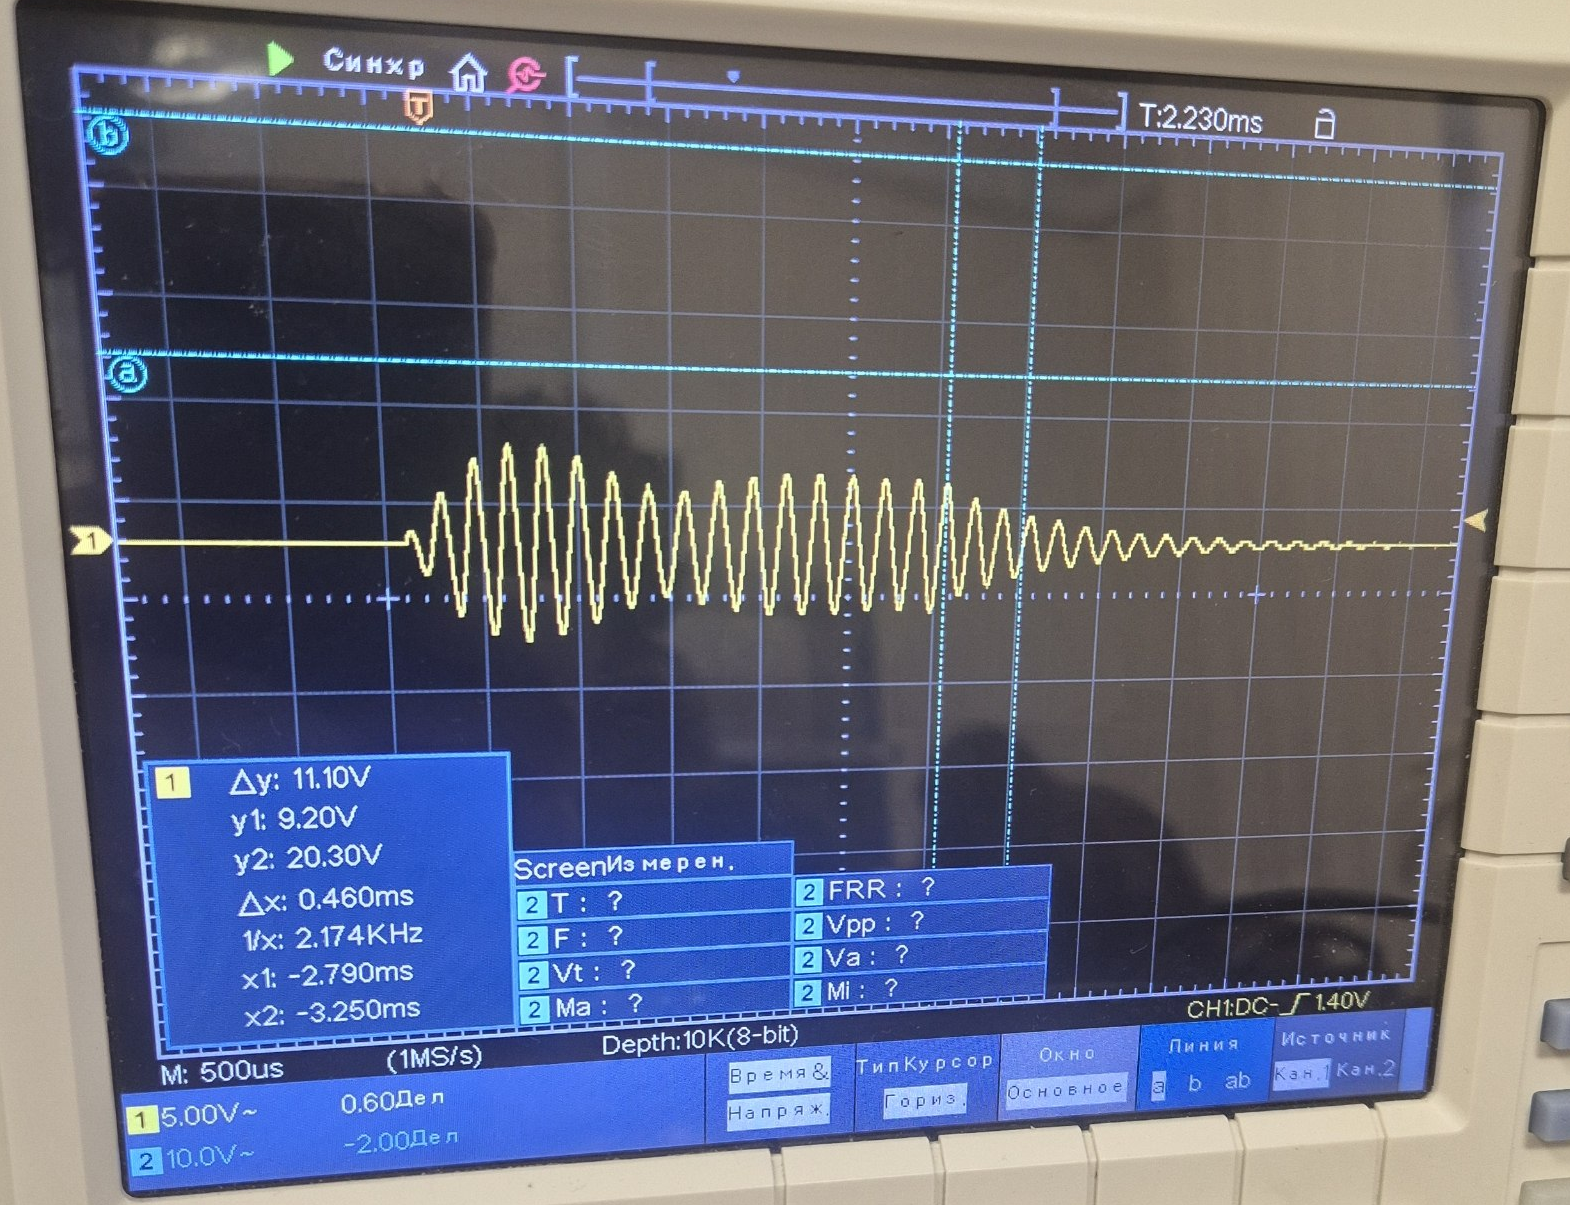
\includegraphics[width=0.85\textwidth]{figures/burst.png}
    \caption{Процессы установления и затухания
    вынужденных колебаний в электрическом контуре}
    \label{fig:burst}
\end{figure}

При подаче цуга синусоидального сигнала амплитуда
колебаний сначала возрастает. Наблюдаемое
немонотонное изменение огибающей связано
с наложением свободных и вынужденных колебаний.
При небольшой расстройке частот их интерференция
может приводить к периодическому усилению
и ослаблению амплитуды.
После прекращения внешнего воздействия
в контуре остаются свободные затухающие
колебания, амплитуда которых убывает
по экспоненциальному закону вследствие
потерь энергии на активном сопротивлении.

\subsection{Наблюдение биений}
При небольшом отклонении частоты генератора от собственной частоты
контура возможно возникновение биений, обусловленных наложением
свободной и вынужденной составляющих с близкими частотами.
Отдельных количественных данных для определения периода биений
в журнале измерений нет.

\subsection{Измерение параметров катушки}
После разборки схемы измерялись активное сопротивление $R_L$
и индуктивность $L$ на трёх частотах.
\begin{table}[H]
\centering\small
\caption{Параметры катушки по данным LCR-метра}
\begin{tabular}{ccc}
\toprule
$\nu$, Гц & $L$, мГн & $R_L$, Ом\\
\midrule
50   & 0,015 & 200,26\\
500  & 0,020 & 200,26\\
1500 & 0,020 & 200,26\\
\bottomrule
\end{tabular}
\end{table}

Значения $L$, записанные по LCR-метру, составляют
$0{,}015$--$0{,}020$ мГн и резко отличаются от установленного
номинала $L=100$ мГн. Единицы измерения необходимо уточнить
по исходным показаниям прибора. До уточнения для расчётов
используется заданное в эксперименте $L=100$ мГн.

\subsection{Оценка погрешностей определения добротности}
Для методов, основанных на логарифмическом декременте,
\[
    Q=\frac{\pi}{\Theta},\qquad
    \sigma_Q=\frac{\pi\sigma_\Theta}{\Theta^2}.
\]

Статистическая погрешность среднего декремента по $N$
повторным определениям оценивалась как
\[
    \sigma_{\overline\Theta}=
    \sqrt{\frac{\sum_{i=1}^{N}(\Theta_i-\overline\Theta)^2}
    {N(N-1)}}.
\]

По разбросу амплитудных оценок нарастающих колебаний получено
\[
    Q_{\text{нар},1}=8{,}09\pm0{,}31,\qquad
    Q_{\text{нар},2}=1{,}79\pm0{,}04.
\]

По разбросу декрементов на участке затухания
\[
    Q_{\text{зат},1}=8{,}05\pm0{,}03,\qquad
    Q_{\text{зат},2}=1{,}798\pm0{,}007.
\]

Для АЧХ и ФЧХ добротность определяется из ширины
частотного интервала $\Delta\nu$ по формуле
\[
    Q=\frac{\nu_0}{\Delta\nu}.
\]

При шаге измерения $0{,}07$ кГц для каждой граничной
частоты принимается оценка неопределённости $0{,}035$ кГц,
поэтому
\[
    \sigma_{\Delta\nu}\approx\sqrt2\cdot0{,}035
    \approx0{,}050\text{ кГц},\qquad
    \sigma_Q\approx Q\frac{\sigma_{\Delta\nu}}{\Delta\nu}.
\]

Получаются приближённые оценки
\[
    Q_{\text{АЧХ},1}=8{,}01\pm0{,}53,\qquad
    Q_{\text{ФЧХ},1}=7{,}95\pm0{,}52.
\]
В случае $R_2$ оценка стандартной ошибки подгонки
параметра $Q$ по табличным точкам даёт
\[
    Q_{\text{АЧХ},2}=2{,}39\pm0{,}04,\qquad
    Q_{\text{ФЧХ},2}=2{,}05\pm0{,}01.
\]
Эти значения характеризуют неопределённость аппроксимации
при выбранной модели и не учитывают приборные ошибки.

Для теоретической добротности
\[
    Q_{\text{теор}}=\frac{1}{R_\Sigma}
        \sqrt{\frac{L}{C_\Sigma}}
\]

при независимых погрешностях параметров имеем
\[
    \frac{\sigma_Q}{Q}=
    \sqrt{\left(\frac{\sigma_{R_\Sigma}}{R_\Sigma}\right)^2+
    \frac14\left(\frac{\sigma_L}{L}\right)^2+
    \frac14\left(\frac{\sigma_{C_\Sigma}}{C_\Sigma}\right)^2}.
\]

Без сведений о точности измерения напряжений, $L$, $C$
и $R_L$ численно определить полную инструментальную
погрешность методов свободного затухания, фазовой спирали
и расчёта по параметрам контура нельзя. Приведённые погрешности
характеризуют статистический разброс либо принятый шаг частоты,
но не суммарную неопределённость измерения.

\newpage

\subsection{Сравнение добротности, определённой различными способами}
Итоговые результаты, вычисленные различными методами, сведены в таблицу.
\begin{table}[H]
\centering
\small
\caption{Добротность контура, определённая различными способами}
\resizebox{\textwidth}{!}{%
\begin{tabular}{cccccccc}
\toprule
& \multicolumn{3}{c}{Свободные колебания}
& \multicolumn{4}{c}{Вынужденные колебания} \\
\cmidrule(lr){2-4}\cmidrule(lr){5-8}
$R$, Ом & $f(L,C,R)$ & $f(\Theta)$ & Спираль
& АЧХ & ФЧХ & Нарастание & Затухание \\
\midrule
400 & 6,27 & 8,02 & 8,07 & 8,01 & 7,95 & 8,09 & 8,05 \\
2000 & 1,71 & 1,97 & н/д & 2,39$^{\dagger}$ & 2,05$^{\dagger}$ & 1,79 & 1,80 \\
\bottomrule
\end{tabular}%
}
\end{table}

\noindent\textit{Примечание.} Обозначение
$\dagger$ относится к результатам, найденным аппроксимацией
табличных АЧХ и ФЧХ, а не непосредственным измерением ширины
кривой. «н/д» --- отдельного результата по фазовой спирали нет.
Для $R=400$ Ом оценки добротности по декременту,
АЧХ, ФЧХ и нарастанию близки к $8$, тогда как
расчёт по номинальным параметрам даёт $Q\approx6{,}27$.
При $R=2000$ Ом оценки по свободному затуханию и по
временному процессу составляют около $1{,}8$--$2{,}0$,
а аппроксимация частотных зависимостей даёт $2{,}39$
и $2{,}05$. По всем методам добротность при увеличении
сопротивления уменьшается.
% ================== ВЫВОД ==================



\section*{Вывод}

В ходе работы были получены следующие результаты:

\begin{itemize}
    \item Собственная ёмкость контура:
    $C_0 = 0{,}00107$ мкФ.

    \item Критическое сопротивление контура:
    $R_{\text{кр}} = 6000$ Ом.
\end{itemize}

При сопротивлении $R_1 = 400$ Ом:

\begin{itemize}
    \item Резонансная частота:
    $\nu_0 = 6{,}012$ кГц.

    \item Резонансная амплитуда:
    $U_0 = 8{,}35$ В.

    \item Добротность по свободным колебаниям:
    $Q_{\text{св}} = 8{,}02$.

    \item Добротность по фазовой спирали:
    $Q_{\text{сп}} = 8{,}07$.

    \item Добротность по АЧХ:
    $Q_{\text{АЧХ}} = 8{,}01$.

    \item Добротность по ФЧХ:
    $Q_{\text{ФЧХ}} = 7{,}95$.

    \item Добротность по нарастанию колебаний:
    $Q_{\text{нар}} = 8{,}09$.

    \item Добротность по затуханию колебаний:
    $Q_{\text{зат}} = 8{,}05$.
\end{itemize}

При сопротивлении $R_2 = 2000$ Ом:

\begin{itemize}
    \item Резонансная частота:
    $\nu_0 = 6{,}000$ кГц.

    \item Резонансная амплитуда:
    $U_0 = 2{,}20$ В.

    \item Добротность по свободным колебаниям:
    $Q_{\text{св}} = 1{,}97$.

    \item Добротность по АЧХ (аппроксимация):
    $Q_{\text{АЧХ}} \approx 2{,}39$.

    \item Добротность по ФЧХ (аппроксимация):
    $Q_{\text{ФЧХ}} \approx 2{,}05$.

    \item Добротность по нарастанию колебаний:
    $Q_{\text{нар}} = 1{,}79$.

    \item Добротность по затуханию колебаний:
    $Q_{\text{зат}} = 1{,}80$.
\end{itemize}


\end{document}
